\documentclass[10pt]{standalone}
\usepackage{pgfplots}
\pgfplotsset{compat=1.15}
\usepackage{mathrsfs}
\usepackage{amssymb}
\usepackage{amsmath}
\usetikzlibrary{arrows}
\pagestyle{empty}

\begin{document}




\tikzset{every picture/.style={line width=0.75pt}} %set default line width to 0.75pt        

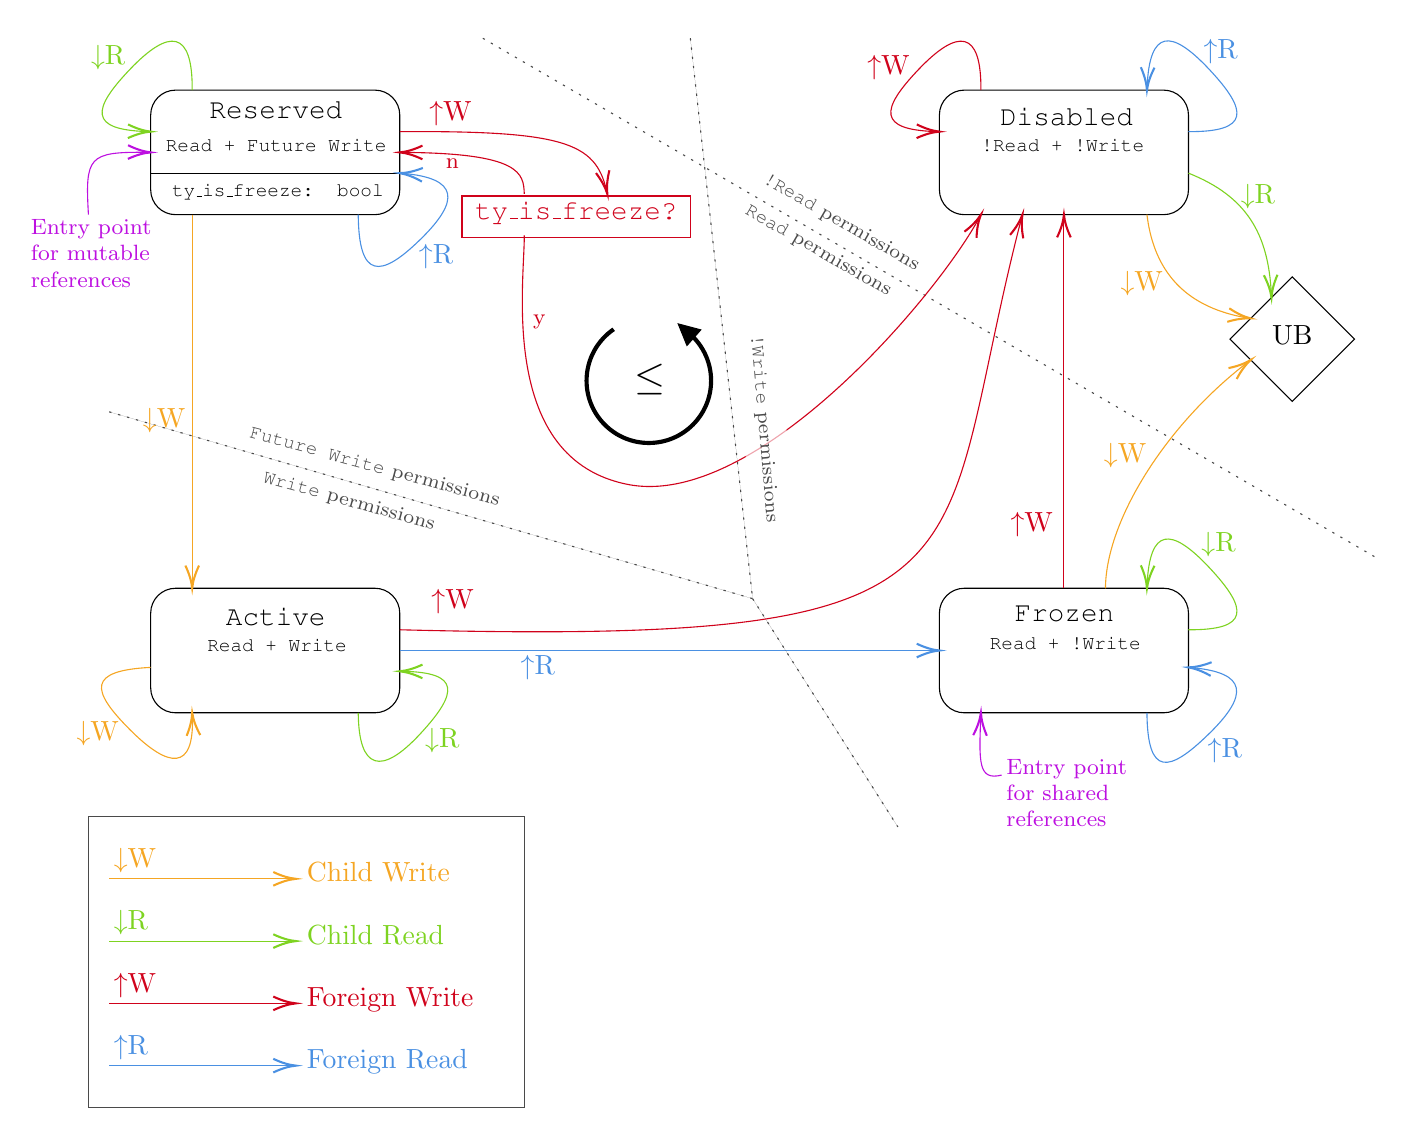
\begin{tikzpicture}[x=0.75pt,y=0.75pt,yscale=-1,xscale=1]
%uncomment if require: \path (0,563); %set diagram left start at 0, and has height of 563

%Rounded Rect [id:dp36193310033866666] 
\draw   (80,72) .. controls (80,65.37) and (85.37,60) .. (92,60) -- (188,60) .. controls (194.63,60) and (200,65.37) .. (200,72) -- (200,108) .. controls (200,114.63) and (194.63,120) .. (188,120) -- (92,120) .. controls (85.37,120) and (80,114.63) .. (80,108) -- cycle ;
%Straight Lines [id:da4928472265000021] 
\draw    (80,100) -- (200,100) ;
%Rounded Rect [id:dp3491373039921244] 
\draw   (80,312) .. controls (80,305.37) and (85.37,300) .. (92,300) -- (188,300) .. controls (194.63,300) and (200,305.37) .. (200,312) -- (200,348) .. controls (200,354.63) and (194.63,360) .. (188,360) -- (92,360) .. controls (85.37,360) and (80,354.63) .. (80,348) -- cycle ;
%Rounded Rect [id:dp9133448241321673] 
\draw   (460,72) .. controls (460,65.37) and (465.37,60) .. (472,60) -- (568,60) .. controls (574.63,60) and (580,65.37) .. (580,72) -- (580,108) .. controls (580,114.63) and (574.63,120) .. (568,120) -- (472,120) .. controls (465.37,120) and (460,114.63) .. (460,108) -- cycle ;
%Rounded Rect [id:dp6976006701742056] 
\draw   (460,312) .. controls (460,305.37) and (465.37,300) .. (472,300) -- (568,300) .. controls (574.63,300) and (580,305.37) .. (580,312) -- (580,348) .. controls (580,354.63) and (574.63,360) .. (568,360) -- (472,360) .. controls (465.37,360) and (460,354.63) .. (460,348) -- cycle ;
%Shape: Rectangle [id:dp4041653725613633] 
\draw  [color={rgb, 255:red, 208; green, 2; blue, 27 }  ,draw opacity=1 ] (230,111) -- (340,111) -- (340,131) -- (230,131) -- cycle ;
%Curve Lines [id:da30918117552924995] 
\draw [color={rgb, 255:red, 208; green, 2; blue, 27 }  ,draw opacity=1 ]   (200,80) .. controls (278.89,79.52) and (294.17,85.22) .. (299.6,108.2) ;
\draw [shift={(300,110)}, rotate = 258.26] [color={rgb, 255:red, 208; green, 2; blue, 27 }  ,draw opacity=1 ][line width=0.75]    (10.93,-3.29) .. controls (6.95,-1.4) and (3.31,-0.3) .. (0,0) .. controls (3.31,0.3) and (6.95,1.4) .. (10.93,3.29)   ;
%Curve Lines [id:da26015823593788967] 
\draw [color={rgb, 255:red, 208; green, 2; blue, 27 }  ,draw opacity=1 ]   (260,110) .. controls (259.58,100.28) and (258.92,90.38) .. (201.75,90.01) ;
\draw [shift={(200,90)}, rotate = 0.17] [color={rgb, 255:red, 208; green, 2; blue, 27 }  ,draw opacity=1 ][line width=0.75]    (10.93,-3.29) .. controls (6.95,-1.4) and (3.31,-0.3) .. (0,0) .. controls (3.31,0.3) and (6.95,1.4) .. (10.93,3.29)   ;
%Straight Lines [id:da6716266791293287] 
\draw [color={rgb, 255:red, 208; green, 2; blue, 27 }  ,draw opacity=1 ]   (520,300) -- (520,122) ;
\draw [shift={(520,120)}, rotate = 90] [color={rgb, 255:red, 208; green, 2; blue, 27 }  ,draw opacity=1 ][line width=0.75]    (10.93,-3.29) .. controls (6.95,-1.4) and (3.31,-0.3) .. (0,0) .. controls (3.31,0.3) and (6.95,1.4) .. (10.93,3.29)   ;
%Straight Lines [id:da8302221098995485] 
\draw [color={rgb, 255:red, 74; green, 144; blue, 226 }  ,draw opacity=1 ]   (200,330) -- (458,330) ;
\draw [shift={(460,330)}, rotate = 180] [color={rgb, 255:red, 74; green, 144; blue, 226 }  ,draw opacity=1 ][line width=0.75]    (10.93,-3.29) .. controls (6.95,-1.4) and (3.31,-0.3) .. (0,0) .. controls (3.31,0.3) and (6.95,1.4) .. (10.93,3.29)   ;
%Shape: Diamond [id:dp2981758453248817] 
\draw   (630,150) -- (660,180) -- (630,210) -- (600,180) -- cycle ;

%Curve Lines [id:da9976874277096126] 
\draw [color={rgb, 255:red, 126; green, 211; blue, 33 }  ,draw opacity=1 ]   (580,100) .. controls (608.33,111.28) and (618.5,129.43) .. (619.92,158.22) ;
\draw [shift={(620,160)}, rotate = 267.91] [color={rgb, 255:red, 126; green, 211; blue, 33 }  ,draw opacity=1 ][line width=0.75]    (10.93,-3.29) .. controls (6.95,-1.4) and (3.31,-0.3) .. (0,0) .. controls (3.31,0.3) and (6.95,1.4) .. (10.93,3.29)   ;
%Curve Lines [id:da36615849055806504] 
\draw [color={rgb, 255:red, 245; green, 166; blue, 35 }  ,draw opacity=1 ]   (560,120) .. controls (562.87,143.82) and (575.2,164.22) .. (608.47,169.76) ;
\draw [shift={(610,170)}, rotate = 188.52] [color={rgb, 255:red, 245; green, 166; blue, 35 }  ,draw opacity=1 ][line width=0.75]    (10.93,-3.29) .. controls (6.95,-1.4) and (3.31,-0.3) .. (0,0) .. controls (3.31,0.3) and (6.95,1.4) .. (10.93,3.29)   ;
%Straight Lines [id:da9454029882711847] 
\draw [color={rgb, 255:red, 245; green, 166; blue, 35 }  ,draw opacity=1 ]   (100,120) -- (100,298) ;
\draw [shift={(100,300)}, rotate = 270] [color={rgb, 255:red, 245; green, 166; blue, 35 }  ,draw opacity=1 ][line width=0.75]    (10.93,-3.29) .. controls (6.95,-1.4) and (3.31,-0.3) .. (0,0) .. controls (3.31,0.3) and (6.95,1.4) .. (10.93,3.29)   ;
%Curve Lines [id:da2730264752893763] 
\draw [color={rgb, 255:red, 245; green, 166; blue, 35 }  ,draw opacity=1 ]   (540,300) .. controls (540.24,267.18) and (569.41,220.94) .. (608.8,190.91) ;
\draw [shift={(610,190)}, rotate = 143.13] [color={rgb, 255:red, 245; green, 166; blue, 35 }  ,draw opacity=1 ][line width=0.75]    (10.93,-3.29) .. controls (6.95,-1.4) and (3.31,-0.3) .. (0,0) .. controls (3.31,0.3) and (6.95,1.4) .. (10.93,3.29)   ;
%Curve Lines [id:da9389496974486098] 
\draw [color={rgb, 255:red, 74; green, 144; blue, 226 }  ,draw opacity=1 ]   (560,360) .. controls (560.24,390.84) and (570.42,389.16) .. (590,370) .. controls (609.19,351.23) and (608.29,340.61) .. (581.66,338.27) ;
\draw [shift={(580,338.13)}, rotate = 4.14] [color={rgb, 255:red, 74; green, 144; blue, 226 }  ,draw opacity=1 ][line width=0.75]    (10.93,-3.29) .. controls (6.95,-1.4) and (3.31,-0.3) .. (0,0) .. controls (3.31,0.3) and (6.95,1.4) .. (10.93,3.29)   ;
%Curve Lines [id:da24128790996830862] 
\draw [color={rgb, 255:red, 126; green, 211; blue, 33 }  ,draw opacity=1 ]   (100,60) .. controls (100.24,30.84) and (88.91,30.18) .. (70,50) .. controls (51.47,69.43) and (50.29,79.12) .. (78.25,79.96) ;
\draw [shift={(80,80)}, rotate = 180.94] [color={rgb, 255:red, 126; green, 211; blue, 33 }  ,draw opacity=1 ][line width=0.75]    (10.93,-3.29) .. controls (6.95,-1.4) and (3.31,-0.3) .. (0,0) .. controls (3.31,0.3) and (6.95,1.4) .. (10.93,3.29)   ;
%Curve Lines [id:da31257438161761253] 
\draw [color={rgb, 255:red, 208; green, 2; blue, 27 }  ,draw opacity=1 ]   (480,60) .. controls (480.24,30.84) and (468.91,30.18) .. (450,50) .. controls (431.47,69.43) and (430.29,79.12) .. (458.25,79.96) ;
\draw [shift={(460,80)}, rotate = 180.94] [color={rgb, 255:red, 208; green, 2; blue, 27 }  ,draw opacity=1 ][line width=0.75]    (10.93,-3.29) .. controls (6.95,-1.4) and (3.31,-0.3) .. (0,0) .. controls (3.31,0.3) and (6.95,1.4) .. (10.93,3.29)   ;
%Curve Lines [id:da11742524855238334] 
\draw [color={rgb, 255:red, 74; green, 144; blue, 226 }  ,draw opacity=1 ]   (580,80) .. controls (609.58,80.18) and (608.91,70.18) .. (590,50) .. controls (571.47,30.23) and (561.32,30.81) .. (560.07,58.28) ;
\draw [shift={(560,60)}, rotate = 271.79] [color={rgb, 255:red, 74; green, 144; blue, 226 }  ,draw opacity=1 ][line width=0.75]    (10.93,-3.29) .. controls (6.95,-1.4) and (3.31,-0.3) .. (0,0) .. controls (3.31,0.3) and (6.95,1.4) .. (10.93,3.29)   ;
%Curve Lines [id:da5812531195082242] 
\draw [color={rgb, 255:red, 126; green, 211; blue, 33 }  ,draw opacity=1 ]   (580,320) .. controls (609.58,320.18) and (608.91,310.18) .. (590,290) .. controls (571.47,270.23) and (561.32,270.81) .. (560.07,298.28) ;
\draw [shift={(560,300)}, rotate = 271.79] [color={rgb, 255:red, 126; green, 211; blue, 33 }  ,draw opacity=1 ][line width=0.75]    (10.93,-3.29) .. controls (6.95,-1.4) and (3.31,-0.3) .. (0,0) .. controls (3.31,0.3) and (6.95,1.4) .. (10.93,3.29)   ;
%Curve Lines [id:da3142098241817616] 
\draw [color={rgb, 255:red, 245; green, 166; blue, 35 }  ,draw opacity=1 ]   (80,338.13) .. controls (49.58,339.64) and (50.91,348.98) .. (70,368.13) .. controls (88.71,386.91) and (101.08,388.26) .. (100.08,361.66) ;
\draw [shift={(100,360)}, rotate = 86.81] [color={rgb, 255:red, 245; green, 166; blue, 35 }  ,draw opacity=1 ][line width=0.75]    (10.93,-3.29) .. controls (6.95,-1.4) and (3.31,-0.3) .. (0,0) .. controls (3.31,0.3) and (6.95,1.4) .. (10.93,3.29)   ;
%Curve Lines [id:da8136035432155564] 
\draw [color={rgb, 255:red, 126; green, 211; blue, 33 }  ,draw opacity=1 ]   (180,360) .. controls (180.24,387.64) and (191.09,390.49) .. (210,370) .. controls (228.53,349.92) and (228.9,340.56) .. (201.7,340.02) ;
\draw [shift={(200,340)}, rotate = 0.35] [color={rgb, 255:red, 126; green, 211; blue, 33 }  ,draw opacity=1 ][line width=0.75]    (10.93,-3.29) .. controls (6.95,-1.4) and (3.31,-0.3) .. (0,0) .. controls (3.31,0.3) and (6.95,1.4) .. (10.93,3.29)   ;
%Straight Lines [id:da925370301171158] 
\draw [color={rgb, 255:red, 126; green, 211; blue, 33 }  ,draw opacity=1 ]   (60,470) -- (148,470) ;
\draw [shift={(150,470)}, rotate = 180] [color={rgb, 255:red, 126; green, 211; blue, 33 }  ,draw opacity=1 ][line width=0.75]    (10.93,-3.29) .. controls (6.95,-1.4) and (3.31,-0.3) .. (0,0) .. controls (3.31,0.3) and (6.95,1.4) .. (10.93,3.29)   ;
%Straight Lines [id:da8542460465559526] 
\draw [color={rgb, 255:red, 245; green, 166; blue, 35 }  ,draw opacity=1 ]   (60,440) -- (148,440) ;
\draw [shift={(150,440)}, rotate = 180] [color={rgb, 255:red, 245; green, 166; blue, 35 }  ,draw opacity=1 ][line width=0.75]    (10.93,-3.29) .. controls (6.95,-1.4) and (3.31,-0.3) .. (0,0) .. controls (3.31,0.3) and (6.95,1.4) .. (10.93,3.29)   ;
%Straight Lines [id:da4752091521246813] 
\draw [color={rgb, 255:red, 208; green, 2; blue, 27 }  ,draw opacity=1 ]   (60,500) -- (148,500) ;
\draw [shift={(150,500)}, rotate = 180] [color={rgb, 255:red, 208; green, 2; blue, 27 }  ,draw opacity=1 ][line width=0.75]    (10.93,-3.29) .. controls (6.95,-1.4) and (3.31,-0.3) .. (0,0) .. controls (3.31,0.3) and (6.95,1.4) .. (10.93,3.29)   ;
%Straight Lines [id:da004195731282831683] 
\draw [color={rgb, 255:red, 74; green, 144; blue, 226 }  ,draw opacity=1 ]   (60,530) -- (148,530) ;
\draw [shift={(150,530)}, rotate = 180] [color={rgb, 255:red, 74; green, 144; blue, 226 }  ,draw opacity=1 ][line width=0.75]    (10.93,-3.29) .. controls (6.95,-1.4) and (3.31,-0.3) .. (0,0) .. controls (3.31,0.3) and (6.95,1.4) .. (10.93,3.29)   ;
%Shape: Rectangle [id:dp15275352306840828] 
\draw  [color={rgb, 255:red, 74; green, 74; blue, 74 }  ,draw opacity=1 ] (50,410) -- (260,410) -- (260,550) -- (50,550) -- cycle ;
%Shape: Arc [id:dp7852510056454136] 
\draw  [draw opacity=0][line width=1.5]  (337.94,175.95) .. controls (345.26,181.43) and (350,190.16) .. (350,200) .. controls (350,216.57) and (336.57,230) .. (320,230) .. controls (303.43,230) and (290,216.57) .. (290,200) .. controls (290,189.71) and (295.18,180.64) .. (303.07,175.23) -- (320,200) -- cycle ; \draw  [line width=1.5]  (337.94,175.95) .. controls (345.26,181.43) and (350,190.16) .. (350,200) .. controls (350,216.57) and (336.57,230) .. (320,230) .. controls (303.43,230) and (290,216.57) .. (290,200) .. controls (290,189.71) and (295.18,180.64) .. (303.07,175.23) ;  
%Shape: Triangle [id:dp6437258532368012] 
\draw  [fill={rgb, 255:red, 0; green, 0; blue, 0 }  ,fill opacity=1 ] (334.19,172.65) -- (345,175.51) -- (338.38,183.01) -- cycle ;
%Curve Lines [id:da1726128897938034] 
\draw [color={rgb, 255:red, 189; green, 16; blue, 224 }  ,draw opacity=1 ]   (50,120) .. controls (48.45,92.12) and (49.7,89.65) .. (78.22,89.98) ;
\draw [shift={(80,90)}, rotate = 180.84] [color={rgb, 255:red, 189; green, 16; blue, 224 }  ,draw opacity=1 ][line width=0.75]    (10.93,-3.29) .. controls (6.95,-1.4) and (3.31,-0.3) .. (0,0) .. controls (3.31,0.3) and (6.95,1.4) .. (10.93,3.29)   ;
%Curve Lines [id:da9756018543015939] 
\draw [color={rgb, 255:red, 189; green, 16; blue, 224 }  ,draw opacity=1 ]   (490,390) .. controls (478.7,392.82) and (479.05,384.01) .. (479.93,361.74) ;
\draw [shift={(480,360)}, rotate = 92.24] [color={rgb, 255:red, 189; green, 16; blue, 224 }  ,draw opacity=1 ][line width=0.75]    (10.93,-3.29) .. controls (6.95,-1.4) and (3.31,-0.3) .. (0,0) .. controls (3.31,0.3) and (6.95,1.4) .. (10.93,3.29)   ;
%Curve Lines [id:da15520907766539005] 
\draw [color={rgb, 255:red, 74; green, 144; blue, 226 }  ,draw opacity=1 ]   (180,120) .. controls (180.24,150.84) and (190.42,151.02) .. (210,131.87) .. controls (229.19,113.09) and (228.29,102.47) .. (201.66,100.13) ;
\draw [shift={(200,100)}, rotate = 4.14] [color={rgb, 255:red, 74; green, 144; blue, 226 }  ,draw opacity=1 ][line width=0.75]    (10.93,-3.29) .. controls (6.95,-1.4) and (3.31,-0.3) .. (0,0) .. controls (3.31,0.3) and (6.95,1.4) .. (10.93,3.29)   ;
%Shape: Rectangle [id:dp5308849319927443] 
\draw  [color={rgb, 255:red, 255; green, 255; blue, 255 }  ,draw opacity=0 ][fill={rgb, 255:red, 255; green, 255; blue, 255 }  ,fill opacity=0.64 ] (129.11,217.54) -- (254.38,256.06) -- (245.3,285.58) -- (120.03,247.07) -- cycle ;
%Straight Lines [id:da5185007165933506] 
\draw [color={rgb, 255:red, 74; green, 74; blue, 74 }  ,draw opacity=1 ][fill={rgb, 255:red, 74; green, 74; blue, 74 }  ,fill opacity=1 ] [dash pattern={on 0.84pt off 2.51pt}]  (60,215) -- (370,305) ;
%Straight Lines [id:da5471872363951132] 
\draw [color={rgb, 255:red, 74; green, 74; blue, 74 }  ,draw opacity=1 ] [dash pattern={on 0.84pt off 2.51pt}]  (240,35) -- (670,285) ;
%Straight Lines [id:da7762316849122682] 
\draw [color={rgb, 255:red, 74; green, 74; blue, 74 }  ,draw opacity=1 ][fill={rgb, 255:red, 74; green, 74; blue, 74 }  ,fill opacity=1 ] [dash pattern={on 0.84pt off 2.51pt}]  (340,35) -- (370,305) ;
%Straight Lines [id:da43903170207206477] 
\draw [color={rgb, 255:red, 74; green, 74; blue, 74 }  ,draw opacity=1 ][fill={rgb, 255:red, 74; green, 74; blue, 74 }  ,fill opacity=1 ] [dash pattern={on 0.84pt off 2.51pt}]  (370,305) -- (440,415) ;
%Curve Lines [id:da717564363988458] 
\draw [color={rgb, 255:red, 208; green, 2; blue, 27 }  ,draw opacity=1 ]   (200,320) .. controls (498.24,327.68) and (454.91,292.34) .. (500,120) ;
\draw [shift={(500,120)}, rotate = 104.66] [color={rgb, 255:red, 208; green, 2; blue, 27 }  ,draw opacity=1 ][line width=0.75]    (10.93,-3.29) .. controls (6.95,-1.4) and (3.31,-0.3) .. (0,0) .. controls (3.31,0.3) and (6.95,1.4) .. (10.93,3.29)   ;
%Curve Lines [id:da8191746458337361] 
\draw [color={rgb, 255:red, 208; green, 2; blue, 27 }  ,draw opacity=1 ]   (260,130) .. controls (260.11,153.48) and (247.6,237.82) .. (310,250) .. controls (371.46,262) and (458.26,159.98) .. (479.09,121.7) ;
\draw [shift={(480,120)}, rotate = 117.39] [color={rgb, 255:red, 208; green, 2; blue, 27 }  ,draw opacity=1 ][line width=0.75]    (10.93,-3.29) .. controls (6.95,-1.4) and (3.31,-0.3) .. (0,0) .. controls (3.31,0.3) and (6.95,1.4) .. (10.93,3.29)   ;
%Shape: Rectangle [id:dp020475036339357877] 
\draw  [color={rgb, 255:red, 255; green, 255; blue, 255 }  ,draw opacity=0 ][fill={rgb, 255:red, 255; green, 255; blue, 255 }  ,fill opacity=0.64 ] (380.84,176.14) -- (391.42,267.61) -- (370.58,270.02) -- (360,178.55) -- cycle ;

% Text Node
\draw (312,191) node [anchor=north west][inner sep=0.75pt]  [font=\Large] [align=left] {$\displaystyle \leq $};
% Text Node
\draw (619,172) node [anchor=north west][inner sep=0.75pt]   [align=left] {UB};
% Text Node
\draw (221,92) node [anchor=north west][inner sep=0.75pt]  [font=\footnotesize,color={rgb, 255:red, 208; green, 2; blue, 27 }  ,opacity=1 ] [align=left] {n};
% Text Node
\draw (263,167) node [anchor=north west][inner sep=0.75pt]  [font=\footnotesize,color={rgb, 255:red, 208; green, 2; blue, 27 }  ,opacity=1 ] [align=left] {y};
% Text Node
\draw (50,37) node [anchor=north west][inner sep=0.75pt]  [color={rgb, 255:red, 126; green, 211; blue, 33 }  ,opacity=1 ] [align=left] {$\displaystyle \downarrow $R};
% Text Node
\draw (546,146) node [anchor=north west][inner sep=0.75pt]  [color={rgb, 255:red, 245; green, 166; blue, 35 }  ,opacity=1 ] [align=left] {$\displaystyle \downarrow $W};
% Text Node
\draw (588,371) node [anchor=north west][inner sep=0.75pt]  [color={rgb, 255:red, 74; green, 144; blue, 226 }  ,opacity=1 ] [align=left] {$\displaystyle \uparrow $R};
% Text Node
\draw (493,262) node [anchor=north west][inner sep=0.75pt]  [color={rgb, 255:red, 208; green, 2; blue, 27 }  ,opacity=1 ] [align=left] {$\displaystyle \uparrow $W};
% Text Node
\draw (424,42) node [anchor=north west][inner sep=0.75pt]  [color={rgb, 255:red, 208; green, 2; blue, 27 }  ,opacity=1 ] [align=left] {$\displaystyle \uparrow $W};
% Text Node
\draw (213,64) node [anchor=north west][inner sep=0.75pt]  [color={rgb, 255:red, 208; green, 2; blue, 27 }  ,opacity=1 ] [align=left] {$\displaystyle \uparrow $W};
% Text Node
\draw (214,299) node [anchor=north west][inner sep=0.75pt]  [color={rgb, 255:red, 208; green, 2; blue, 27 }  ,opacity=1 ] [align=left] {$\displaystyle \uparrow $W};
% Text Node
\draw (586,34) node [anchor=north west][inner sep=0.75pt]  [color={rgb, 255:red, 74; green, 144; blue, 226 }  ,opacity=1 ] [align=left] {$\displaystyle \uparrow $R};
% Text Node
\draw (257,331) node [anchor=north west][inner sep=0.75pt]  [color={rgb, 255:red, 74; green, 144; blue, 226 }  ,opacity=1 ] [align=left] {$\displaystyle \uparrow $R};
% Text Node
\draw (538,229) node [anchor=north west][inner sep=0.75pt]  [color={rgb, 255:red, 245; green, 166; blue, 35 }  ,opacity=1 ] [align=left] {$\displaystyle \downarrow $W};
% Text Node
\draw (43,363) node [anchor=north west][inner sep=0.75pt]  [color={rgb, 255:red, 245; green, 166; blue, 35 }  ,opacity=1 ] [align=left] {$\displaystyle \downarrow $W};
% Text Node
\draw (75,212) node [anchor=north west][inner sep=0.75pt]  [color={rgb, 255:red, 245; green, 166; blue, 35 }  ,opacity=1 ] [align=left] {$\displaystyle \downarrow $W};
% Text Node
\draw (211,366) node [anchor=north west][inner sep=0.75pt]  [color={rgb, 255:red, 126; green, 211; blue, 33 }  ,opacity=1 ] [align=left] {$\displaystyle \downarrow $R};
% Text Node
\draw (604,104) node [anchor=north west][inner sep=0.75pt]  [color={rgb, 255:red, 126; green, 211; blue, 33 }  ,opacity=1 ] [align=left] {$\displaystyle \downarrow $R};
% Text Node
\draw (585,272) node [anchor=north west][inner sep=0.75pt]  [color={rgb, 255:red, 126; green, 211; blue, 33 }  ,opacity=1 ] [align=left] {$\displaystyle \downarrow $R};
% Text Node
\draw (61,424) node [anchor=north west][inner sep=0.75pt]  [color={rgb, 255:red, 245; green, 166; blue, 35 }  ,opacity=1 ] [align=left] {$\displaystyle \downarrow $W};
% Text Node
\draw (61,454) node [anchor=north west][inner sep=0.75pt]  [color={rgb, 255:red, 126; green, 211; blue, 33 }  ,opacity=1 ] [align=left] {$\displaystyle \downarrow $R};
% Text Node
\draw (61,514) node [anchor=north west][inner sep=0.75pt]  [color={rgb, 255:red, 74; green, 144; blue, 226 }  ,opacity=1 ] [align=left] {$\displaystyle \uparrow $R};
% Text Node
\draw (61,484) node [anchor=north west][inner sep=0.75pt]  [color={rgb, 255:red, 208; green, 2; blue, 27 }  ,opacity=1 ] [align=left] {$\displaystyle \uparrow $W};
% Text Node
\draw (154,431) node [anchor=north west][inner sep=0.75pt]  [color={rgb, 255:red, 245; green, 166; blue, 35 }  ,opacity=1 ] [align=left] {Child Write};
% Text Node
\draw (154,461) node [anchor=north west][inner sep=0.75pt]  [color={rgb, 255:red, 126; green, 211; blue, 33 }  ,opacity=1 ] [align=left] {Child Read};
% Text Node
\draw (154,491) node [anchor=north west][inner sep=0.75pt]  [color={rgb, 255:red, 208; green, 2; blue, 27 }  ,opacity=1 ] [align=left] {Foreign Write};
% Text Node
\draw (154,521) node [anchor=north west][inner sep=0.75pt]  [color={rgb, 255:red, 74; green, 144; blue, 226 }  ,opacity=1 ] [align=left] {Foreign Read};
% Text Node
\draw (89.06,104) node [anchor=north west][inner sep=0.75pt]  [font=\scriptsize] [align=left] {{\fontfamily{pcr}\selectfont ty\_is\_freeze: bool}};
% Text Node
\draw (107.06,64) node [anchor=north west][inner sep=0.75pt]   [align=left] {{\fontfamily{pcr}\selectfont Reserved}};
% Text Node
\draw (115,308) node [anchor=north west][inner sep=0.75pt]   [align=left] {{\fontfamily{pcr}\selectfont Active}};
% Text Node
\draw (488,67) node [anchor=north west][inner sep=0.75pt]   [align=left] {{\fontfamily{pcr}\selectfont Disabled}};
% Text Node
\draw (495,307) node [anchor=north west][inner sep=0.75pt]   [align=left] {{\fontfamily{pcr}\selectfont Frozen}};
% Text Node
\draw (21,121) node [anchor=north west][inner sep=0.75pt]  [font=\footnotesize,color={rgb, 255:red, 189; green, 16; blue, 224 }  ,opacity=1 ] [align=left] {Entry point\\for mutable\\references};
% Text Node
\draw (491,381) node [anchor=north west][inner sep=0.75pt]  [font=\footnotesize,color={rgb, 255:red, 189; green, 16; blue, 224 }  ,opacity=1 ] [align=left] {Entry point\\for shared\\references};
% Text Node
\draw (235,112) node [anchor=north west][inner sep=0.75pt]  [color={rgb, 255:red, 208; green, 2; blue, 27 }  ,opacity=1 ] [align=left] {{\fontfamily{pcr}\selectfont ty\_is\_freeze?}};
% Text Node
\draw (208,132.87) node [anchor=north west][inner sep=0.75pt]  [color={rgb, 255:red, 74; green, 144; blue, 226 }  ,opacity=1 ] [align=left] {$\displaystyle \uparrow $R};
% Text Node
\draw (86,82) node [anchor=north west][inner sep=0.75pt]  [font=\scriptsize] [align=left] {{\fontfamily{pcr}\selectfont Read + Future Write}};
% Text Node
\draw (479,82) node [anchor=north west][inner sep=0.75pt]  [font=\scriptsize] [align=left] {{\fontfamily{pcr}\selectfont !Read + !Write}};
% Text Node
\draw (483,322) node [anchor=north west][inner sep=0.75pt]  [font=\scriptsize] [align=left] {{\fontfamily{pcr}\selectfont Read + !Write}};
% Text Node
\draw (106,323) node [anchor=north west][inner sep=0.75pt]  [font=\scriptsize] [align=left] {{\fontfamily{pcr}\selectfont Read + Write}};
% Text Node
\draw (134.76,241.37) node [anchor=north west][inner sep=0.75pt]  [font=\scriptsize,color={rgb, 255:red, 74; green, 74; blue, 74 }  ,opacity=1 ,rotate=-15.56] [align=left] {{\fontfamily{pcr}\selectfont Write} permissions};
% Text Node
\draw (368.71,112.23) node [anchor=north west][inner sep=0.75pt]  [font=\scriptsize,color={rgb, 255:red, 74; green, 74; blue, 74 }  ,opacity=1 ,rotate=-30.07] [align=left] {{\fontfamily{pcr}\selectfont Read} permissions};
% Text Node
\draw (377.38,97.23) node [anchor=north west][inner sep=0.75pt]  [font=\scriptsize,color={rgb, 255:red, 74; green, 74; blue, 74 }  ,opacity=1 ,rotate=-30.07] [align=left] {{\fontfamily{pcr}\selectfont !Read} permissions};
% Text Node
\draw (376.73,176.16) node [anchor=north west][inner sep=0.75pt]  [font=\scriptsize,color={rgb, 255:red, 74; green, 74; blue, 74 }  ,opacity=1 ,rotate=-85.19] [align=left] {{\fontfamily{pcr}\selectfont !Write} permissions};
% Text Node
\draw (128.05,219.83) node [anchor=north west][inner sep=0.75pt]  [font=\scriptsize,color={rgb, 255:red, 74; green, 74; blue, 74 }  ,opacity=1 ,rotate=-15.22] [align=left] {{\fontfamily{pcr}\selectfont Future Write} permissions};


\end{tikzpicture}


\end{document}
